\documentclass{article}
\author{Wenzhao Xu, Haoyan Cai}
\title{STAT 542 Final Project Proposal}
\usepackage{amsmath}
\usepackage{graphicx}
\usepackage{subfig}
\usepackage{multirow}
\usepackage[top=1in, bottom=1in, left=1.25in, right=1.25in]{geometry}

\begin{document}
	\maketitle
	
	\section{Introduction} % (fold)
	\label{sec:introduction}
	
	\paragraph{} The data are about accelerometer data from mobile device. The train data contain X,Y,Z acceleration data from 387 devices and testing data set have 90024 testing sequences. In addition, for each test sequence, we have information of a possible device. The goal is to judge whether this possible device is the true device that generate the test sequence. 
	
	% section introduction (end)
	
	\section{Data Set} % (fold)
	\label{sec:section_name}
	Package "ff" is used to extract data from a large csv file and unix time is converted to GMT time. There are totally 387 training devices, and 90024 testing sequences. A typical visulization of data is shown in Figure 1, in which Device 7 is a device with long sampling time and total 523187 points while Device 770 has limited sampling points as 28475.
	\begin{figure}
		\centering
		\subfloat[Device 770]{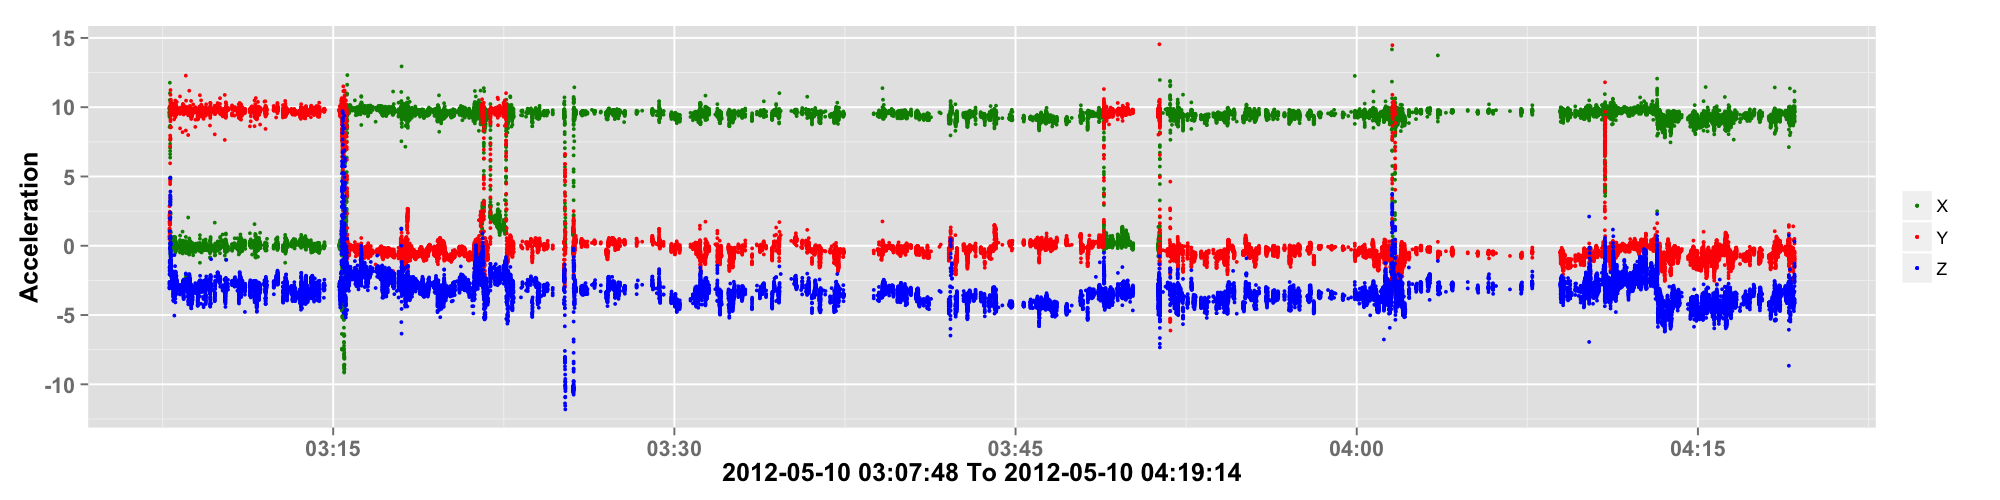
\includegraphics[width=1\textwidth]{photoshare/770.png}}\\
		\subfloat[Device 7]{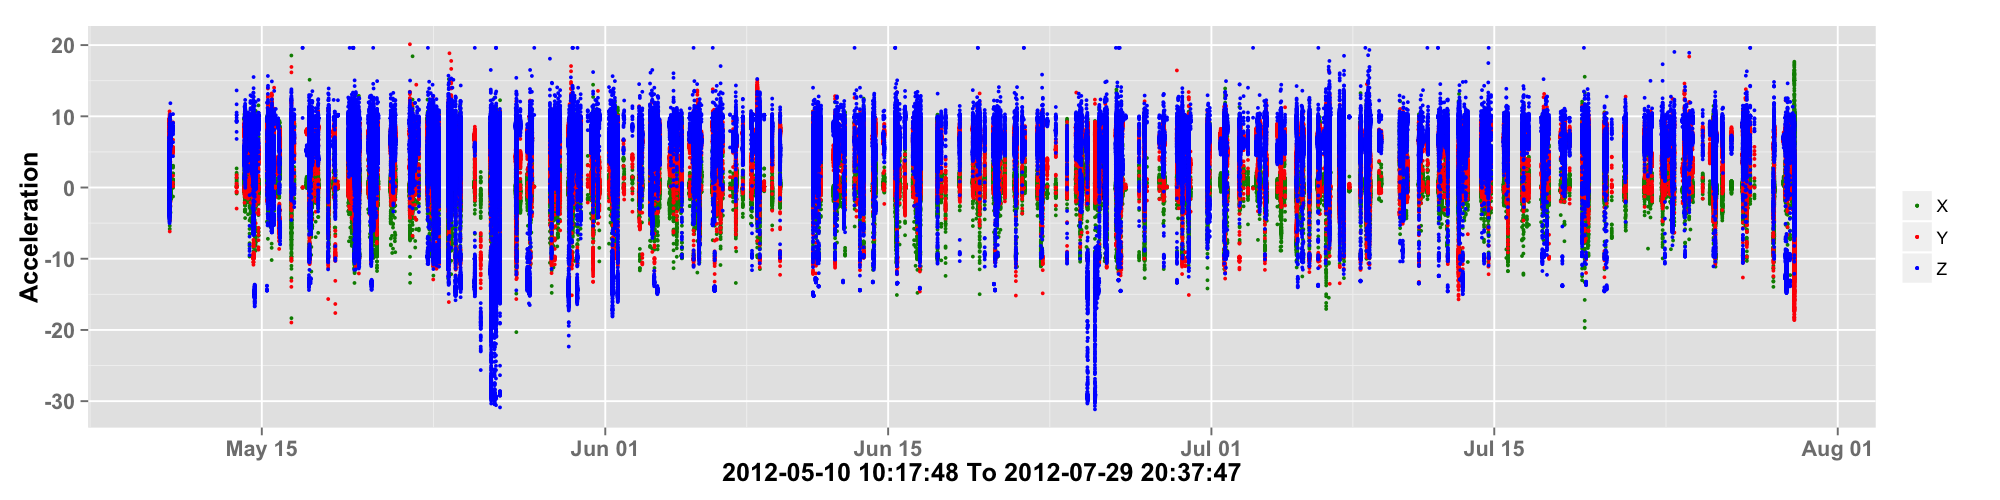
\includegraphics[width=1\textwidth]{photoshare/7.png}} \\
		\caption{Acceleration Data Along Time}
	\end{figure}
	
	\paragraph{}In test data, we need to identify the professed device is the true number. Figure 2 shows two sequence whose professed device is 770. Compared with the train data with device 770, it seems sequence 838966 is likely belong to Device 770 while sequence 690194 is not since the range of X,Y,Z in sequence 838966 is in consistnace with training data of device 770. 
	\begin{figure}
		\centering
		\subfloat[Sequence 690194]{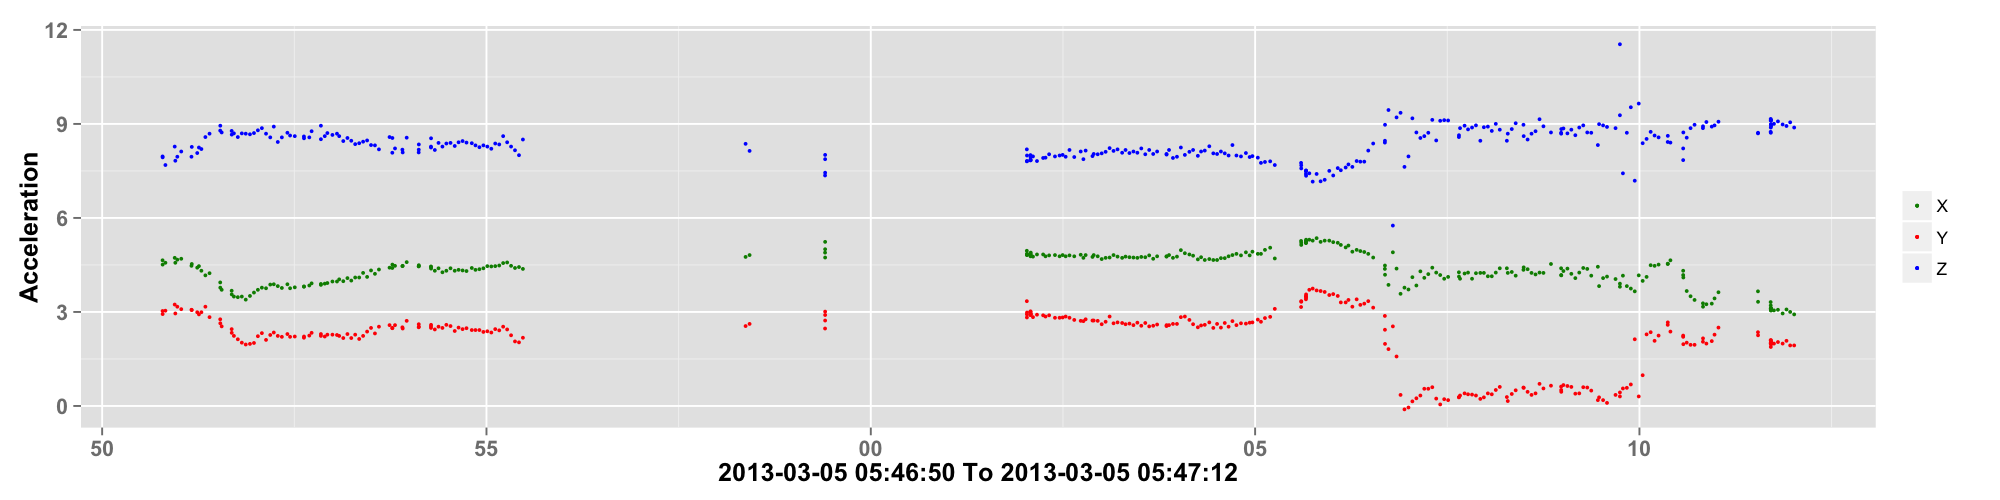
\includegraphics[width=1\textwidth]{photoshare/690194.png}}\\
		\subfloat[Sequence 838966]{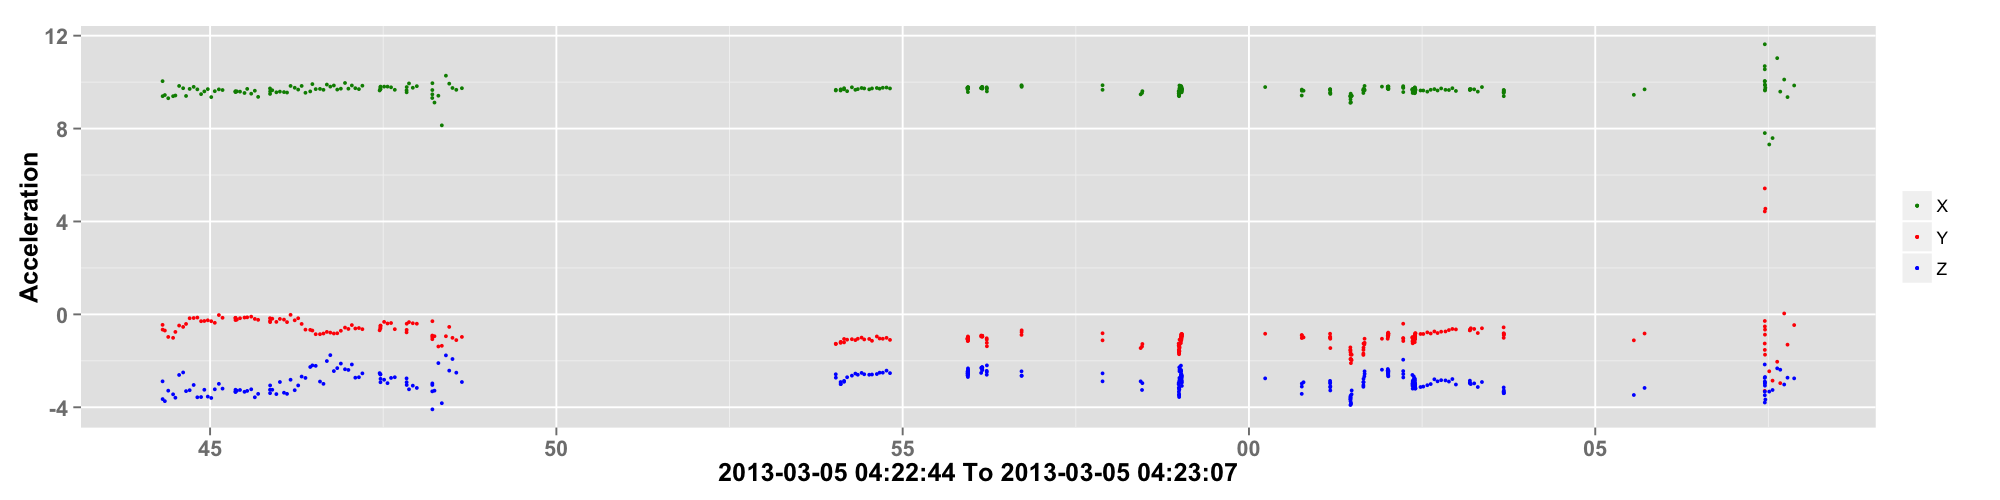
\includegraphics[width=1\textwidth]{photoshare/838966.png}}
		\caption{Test Sequence with Professed Device as 770}
	\end{figure}
	
	% section section_name (end)
	

	
	\section{Potential Approach} % (fold)
	\label{sec:potential_approach}
	\paragraph{}The data involve with time dimension, which is a very important feature. First, we need to define features from the raw data. Some simple but might be useful features include the range of X,Y,Z, the difference between X and Y, between X and Z, and between Y and Z, autocorrelation of X,Y and Z, and correlations between X,Y and Z, etc. We plan to do some literature research about what activities the data might reveal in order to extact features that represent users personal habbit such as how he/she runs. Then,an assumption should be made that users activities have similarity. Similarity means users are likely to have similar behavoir during similar time of day. For example, users would have similary X,Y and Z time series during today's 4:00pm and during yesterday's 4:00pm. 
	
	\paragraph{} One big problem is that how we define the probability for a test sequence to be rejected. First, since data are generated by different time, training data might have different patterns during different time period. Given a test sequence, denote its day time period as $T_{test}$. Then search all the training data and extract the data that generated at the similar day time. For a test sequence, a professed device $D$ is known. So we can label the data from device $D$ as 1 and the data from other device as 0. Train the model with these training data and get the classifier. Then fit the test sequence to see wether it is 0 (test sequence is belong to other device) or 1 (test sequence is belong to device $D$). If possible, identify what activity the test sequence represents such as running or walking or sleeping. If the test sequence is from running,then find the device with similar running patterns.
	
	% section potential_approach (end)
	
\end{document}




